% ====================================================================
% v4-02.tex — Chapter 2 (v4: 통계열역학 챕터, 분포 명시 전개)
%   ★v4 = 격자기체 분배함수 → 점유 분포 → S_config/vib/electronic 엔트로피
%         → 섞임/겹침 수식 → 가역 발열. 코인 하프셀(흑연 음극 vs Li) 단독.
%         v3 Bernardi 틀 보존·심화. 전셀 합성 범위 외.
%   build: xelatex 2-pass (kotex). 0-error 목표.
%   작가: v4-02 (Sonnet, 경쟁 빌드)
% ====================================================================
\documentclass[11pt,a4paper]{article}
\usepackage[margin=22mm]{geometry}
\usepackage{kotex}
\setmonofont{D2Coding}[Scale=MatchLowercase]
\usepackage{amsmath,amssymb,mathtools,bm}
\usepackage{booktabs,longtable,array}
\usepackage{enumitem}
\usepackage{amsthm}
\usepackage{hyperref}
\usepackage{fancyhdr}
\usepackage{lastpage}
\usepackage{setspace}
\usepackage{tikz}
\usetikzlibrary{arrows.meta,calc,decorations.pathreplacing}
\setstretch{1.12}
\setlength{\parskip}{0.45em}\setlength{\parindent}{0pt}\setlength{\headheight}{14pt}
\setlength{\emergencystretch}{2em}
\hypersetup{colorlinks=true, linkcolor=blue, urlcolor=blue, citecolor=blue,
  pdftitle={흑연 음극 dQ/dV — Chapter 2 (v4): 엔트로피·가역 발열 통계열역학}}
\pagestyle{fancy}\fancyhf{}
\lhead{흑연 음극 $dQ/dV$ — Ch.\,2 (v4, 통계열역학 분포 전개)}\rhead{\thepage/\pageref{LastPage}}
\renewcommand{\headrulewidth}{0.4pt}
\newtheorem*{keybox}{핵심}
\newtheorem*{srcbox}{문헌 근거}
\newtheorem*{warnbox}{주의}
\newtheorem*{derivebox}{유도}
\newcommand{\dd}{\mathrm{d}}
\newcommand{\rxn}{\mathrm{rxn}}
\newcommand{\eq}{\mathrm{eq}}
\newcommand{\rev}{\mathrm{rev}}
\newcommand{\irr}{\mathrm{irr}}
\newcommand{\oc}{\mathrm{oc}}
\newcommand{\config}{\mathrm{config}}
\newcommand{\vib}{\mathrm{vib}}
\newcommand{\elec}{\mathrm{e}}
\newcommand{\eff}{\mathrm{eff}}
\newcommand{\hys}{\mathrm{hys}}
\renewcommand{\theequation}{2.\arabic{equation}}
\renewcommand{\thesection}{2.\arabic{section}}
\title{\textbf{\LARGE Chapter 2}\\[0.35em]
  \Large 흑연 음극 $dQ/dV$ 의 엔트로피와 가역 발열\\[0.2em]
  \large --- 격자기체 분포에서 $\partial U/\partial T$\,·$\,\Delta S(x)$\,·$\,\dot Q_\rev$ 로 (v4)}
\author{}\date{}

\begin{document}
\maketitle
\tableofcontents
\bigskip

% ====================================================================
\section*{서 — 분포 없이 엔트로피를 다룰 수 없는 이유}
\addcontentsline{toc}{section}{서}
% ====================================================================

Chapter~1 은 흑연 음극의 $\dd Q/\dd V$ 를, 전이별 평형 중심 전위
$U_j(T)=(-\Delta H_{\rxn,j}+T\,\Delta S_{\rxn,j})/F$ 에 세운 logistic 종(種)과
그 위에 얹힌 동역학 꼬리로 기술했다. 이 장(Chapter~2)은 \emph{새 물리를 도입하지
않는다}. 대신, Chapter~1 의 구조가 \emph{왜} 그 모양인지 --- 분포(distribution)의
언어로 --- 를 밝힌다.

핵심 주장은 다음 세 문장이다.
\begin{enumerate}[leftmargin=1.6em,itemsep=3pt]
\item 격자기체(lattice-gas) 분배함수에서 유도한 \textbf{점유 분포}(grand-canonical
  단일-자리 Fermi 함수)가 Chapter~1 의 logistic 식과 수학적으로 동일하다.
\item 이 분포의 Shannon/Boltzmann 엔트로피가 \textbf{configurational 엔트로피}
  $S_\config=-R[\theta\ln\theta+(1-\theta)\ln(1-\theta)]$ 를 주며, 그 부분몰 도함수가
  $\partial U/\partial T$ 의 봉우리-내부($x$-의존) 항이다.
\item 따라서 관측 엔트로피 계수 $\partial U_\oc/\partial T(x)$ 는 세 분포(격자기체
  config\,·\,포논 Bose--Einstein\,·\,전자 Fermi--Dirac)가 합산한 값이고,
  가역 발열 $\dot Q_\rev=-IT\,\partial U/\partial T$ 는 \emph{분포를 재배열하는 열}이다.
\end{enumerate}

이 구조 위에서 겹침 가중식(파생~A), 이중계산 금지(파생~B), 상호작용 유효 폭
$w_\eff(\Omega)$(파생~C), 히스테리시스 분기(파생~D), 극한 검산(파생~I) 을 순서대로
닫는다. 범위는 \textbf{코인 하프셀(흑연 음극 vs Li 금속, 단일 전극)에 한정}한다 ---
전셀 합성($\partial U_\text{cell}=\partial U_\text{cat}-\partial U_\text{an}$)은 이 장의
범위 밖이다.

% ====================================================================
\section{가역열과 비가역열 — Bernardi 에너지 수지}\label{sec:bernardi}
% ====================================================================

전지 셀의 발열은 가역(reversible, 엔트로피) 성분과 비가역(irreversible) 성분으로
나뉜다. Bernardi, Pawlikowski, Newman~\cite{bernardi1985} 의 일반 에너지 수지에서,
부반응·혼합·상변화를 무시한 단일 활물질 한계의 발열률은
\begin{equation}
  \dot Q \;=\; I\,(U_\oc-V) \;-\; I\,T\,\frac{\partial U_\oc}{\partial T}\,,
  \label{eq:bernardi}
\end{equation}
이다($I>0$ 방전, $V$ 단자 전압, $U_\oc$ 개방회로 전위). 우변 첫 항은
비가역열($\dot Q_\irr=I\eta\ge0$, 과전압 소산), 둘째 항이 \textbf{가역열}
\begin{equation}
  \boxed{\;\dot Q_\rev \;=\; -\,I\,T\,\dfrac{\partial U_\oc}{\partial T}\;,}
  \label{eq:qrev}
\end{equation}
이며 $\partial U_\oc/\partial T$ 의 부호에 따라 흡열 또는 발열이 교대한다.

\begin{srcbox}
평형 전위와 반응 깁스 에너지는 $\Delta G=-nFU_\oc$ 로 묶이고,
$\Delta S=-\partial(\Delta G)/\partial T$ 에서 $\Delta S=+nF\,\partial U_\oc/\partial T$
가 나온다. 따라서
$\dot Q_\rev=-IT\,\partial U/\partial T=-(I/nF)\,T\,\Delta S$
다~\cite{newman2004,msmr_partI}. 부호 규약: 본 장은 음극 평형 전위 $U_\oc$ 기준
$\Delta S=+F\,\partial U/\partial T$ 로 통일한다.
\end{srcbox}

이 장의 목표는 식~\eqref{eq:qrev} 의 $\partial U_\oc/\partial T(x)$ 를
\emph{격자기체 분포로부터 닫힌식으로 세우는 것}이다. 그러자면 점유 확률 분포
$\xi_j(U,T)$ 의 통계역학적 기원을 명시해야 한다.

% ====================================================================
\section{격자기체 분배함수와 점유 분포}\label{sec:partition}
% ====================================================================

\subsection{단일 자리 — grand-canonical 2-상태계}

흑연 격자의 자리 하나가 빈 상태($\varepsilon=0$)이거나 Li 이온이 점유한 상태
($\varepsilon=\varepsilon_0$)에 있다고 하자. 화학 퍼텐셜 $\mu$ 와 열평형인
grand-canonical 앙상블에서 분배함수는
\begin{equation}
  Z_1 \;=\; 1 \;+\; e^{-\beta(\varepsilon_0-\mu)},
  \qquad \beta\equiv\frac{1}{k_BT}\,.
  \label{eq:Z1}
\end{equation}
평균 점유수(점유 확률)는
\begin{equation}
  \langle n\rangle \;=\; -\frac{\partial\ln Z_1}{\partial(\beta\varepsilon_0)}
  \;=\; \frac{e^{-\beta(\varepsilon_0-\mu)}}{1+e^{-\beta(\varepsilon_0-\mu)}}
  \;=\; \frac{1}{1+e^{\beta(\varepsilon_0-\mu)}}\,.
  \label{eq:fd_raw}
\end{equation}
이것은 입자 에너지 $\varepsilon_0$, 화학 퍼텐셜 $\mu$ 인 Fermi--Dirac 분포와
구조가 동일하다(자리당 2-상태).

\subsection{Ch1 logistic의 기원}

전기화학 맥락에서 $\varepsilon_0-\mu$ 를 전기화학 퍼텐셜로 치환한다. 전이 $j$ 에서
Li 이온을 삽입하는 반응의 평형 조건은
$\mu_{\mathrm{Li}}=U_j F$ (vs.\,Li/Li$^+$, $n=1$)이고,
$\beta(\varepsilon_0-\mu)=(\varepsilon_0-\mu_{\mathrm{Li}})/k_BT$
를 $\sigma_d(V-U_j)/w_j$ ($w_j\equiv RT/F$) 로 쓰면,
\begin{equation}
  \xi_{\eq,j}(V,T) \;=\; \langle n\rangle \;=\;
  \frac{1}{1+e^{-\sigma_d(V-U_j)/w_j}}\,,
  \label{eq:logistic_origin}
\end{equation}
여기서 $\sigma_d=\pm1$ 은 전이 방향, $U_j(T)=(-\Delta H_{\rxn,j}+T\Delta S_{\rxn,j})/F$
는 Chapter~1 의 전이 중심이다.

\begin{keybox}
\textbf{Ch1 logistic = 격자기체 grand-canonical 점유 분포.}
식~\eqref{eq:logistic_origin}은 식~\eqref{eq:fd_raw} 와 수학적으로 동일하다.
Chapter~1 의 logistic 폭 $w=RT/F$ 는 열에너지 $k_BT$ 를 전기화학 단위(V)로
환산한 것이다 --- 폭이 넓을수록 분포가 더 넓게 퍼진다.
\end{keybox}

\subsection{다자리 평균장 — Bragg--Williams 확장}

자리 간 Li--Li 상호작용을 평균장 수준에서 고려하면(Bragg--Williams),
몰당 깁스 에너지는
\begin{equation}
  g(\theta) \;=\; g_0 + RT\bigl[\theta\ln\theta+(1-\theta)\ln(1-\theta)\bigr]
  + \Omega\,\theta(1-\theta)\,,
  \label{eq:BW}
\end{equation}
여기서 $\theta\in[0,1]$ 은 총 자리 분율 점유율, $\Omega$ 는 몰당 상호작용 에너지
(인력 $\Omega<0$, 척력 $\Omega>0$)이다. 첫째 항은 기준, 둘째 항은 \emph{혼합 자유
에너지}(분포 기여, \S\ref{sec:config} 에서 자세히), 셋째 항은 상호작용 에너지이다.
$\Omega>2RT$ 이면 $g(\theta)$ 가 쌍봉이 되어 상분리(bimodal 공존)가 일어난다.

\begin{figure}[h]
\centering
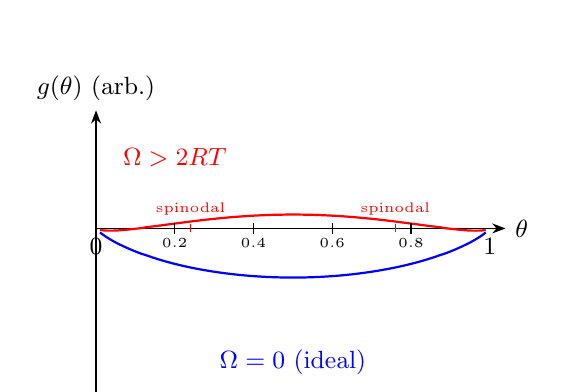
\begin{tikzpicture}[>=Stealth, font=\small]
  % Axes
  \draw[->] (0,0) -- (5.2,0) node[right] {$\theta$};
  \draw[->] (0,-2.2) -- (0,1.5) node[above] {$g(\theta)$ (arb.)};
  % Tick labels
  \node[below] at (0,0) {$0$};
  \node[below] at (5,0) {$1$};
  % Omega=0 curve (pure configurational mixing, convex => concave = mixing lowers G)
  \draw[blue,thick,domain=0.05:4.95,samples=120]
    plot (\x, {0.9*((\x/5)*ln(\x/5) + (1-\x/5)*ln(1-\x/5))});
  \node[blue] at (2.5,-1.7) {$\Omega=0$ (ideal)};
  % Omega>2RT curve (bimodal => concave up in middle)
  \draw[red,thick,domain=0.05:4.95,samples=120]
    plot (\x, {0.9*((\x/5)*ln(\x/5)+(1-\x/5)*ln(1-\x/5))
               + 3.2*(\x/5)*(1-\x/5)});
  \node[red] at (1.0,0.9) {$\Omega>2RT$};
  % Mark spinodal region
  \draw[red,dashed] (1.2,-0.05) -- (1.2,0.05) node[above,red,font=\tiny]{spinodal};
  \draw[red,dashed] (3.8,-0.05) -- (3.8,0.05) node[above,red,font=\tiny]{spinodal};
  % Axis ticks
  \foreach \x in {1,2,3,4} \draw (\x,-0.07)--(\x,0.07);
  \foreach \x in {0.2,0.4,0.6,0.8} \node[below,font=\tiny] at (5*\x,0) {$\x$};
\end{tikzpicture}
\caption{Bragg--Williams 몰 깁스 에너지 $g(\theta)$. 이상 혼합($\Omega=0$, 파란선)은 오목하여
  ($\partial^2 g/\partial\theta^2>0$, 단상 안정). $\Omega>2RT$ (빨간선)는 중간 구간에서 볼록($\partial^2 g/\partial\theta^2<0$),
  두 spinodal 사이에서 상분리가 자발적으로 발생한다.}
\label{fig:BW_g}
\end{figure}

% ====================================================================
\section{분포에서 configurational 엔트로피로}\label{sec:config}
% ====================================================================

\subsection{Shannon--Boltzmann 공식}

격자 자리 $i$ 의 점유 확률이 $p_i=\theta$(점유) 또는 $1-\theta$(빈) 인 두-상태
분포의 Shannon 엔트로피(Boltzmann 공식)는
\begin{equation}
  S_\config \;=\; -R\sum_i p_i\ln p_i
  \;=\; -R\bigl[\theta\ln\theta+(1-\theta)\ln(1-\theta)\bigr]
  \qquad (\text{자리 1몰당})\,.
  \label{eq:Sconfig}
\end{equation}
$S_\config\ge0$, $\theta=0$ 또는 $1$ 에서 $S_\config=0$(완전 정렬),
$\theta=1/2$ 에서 $S_\config=R\ln2$(최대 무질서).

\begin{figure}[h]
\centering
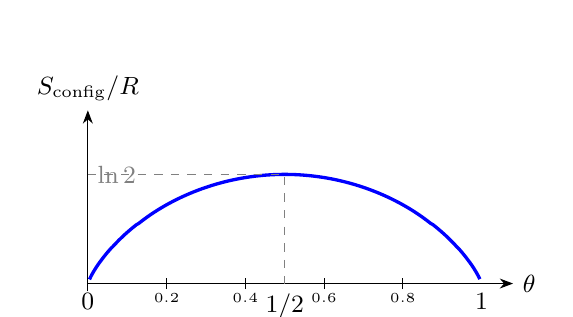
\begin{tikzpicture}[>=Stealth,font=\small]
  \draw[->] (0,0) -- (5.4,0) node[right] {$\theta$};
  \draw[->] (0,-0.1) -- (0,2.2) node[above] {$S_\config/R$};
  \draw[blue,very thick,domain=0.02:4.98,samples=200]
    plot(\x, {-((\x/5)*ln(\x/5)+(1-\x/5)*ln(1-\x/5))*2.0});
  % ln(2) mark
  \draw[dashed,gray] (0,{2*ln(2)}) -- (2.5,{2*ln(2)}) -- (2.5,0);
  \node[right,gray] at (0,{2*ln(2)}) {$\ln 2$};
  \node[below] at (2.5,0) {$1/2$};
  \foreach \x in {0.2,0.4,0.6,0.8} \node[below,font=\tiny] at (5*\x,0) {$\x$};
  \node[below] at (0,0) {$0$}; \node[below] at (5,0) {$1$};
  \foreach \x in {1,2,3,4} \draw (\x,-0.07)--(\x,0.07);
\end{tikzpicture}
\caption{몰 configurational 엔트로피 $S_\config/R=-[\theta\ln\theta+(1-\theta)\ln(1-\theta)]$.
  $\theta=0,1$ (완전 정렬)에서 0, $\theta=1/2$ (최대 혼합)에서 $\ln 2=0.693$ 로 최대.
  부분몰 도함수 $\partial S_\config/\partial\theta=-R\ln[\theta/(1-\theta)]$ 는 양 극한서 발산한다.}
\label{fig:Sconfig}
\end{figure}

\subsection{부분몰 엔트로피 — $\partial U/\partial T$ 의 봉우리-내부 항}

$S_\config$ 를 $\theta$ 로 편미분하면
\begin{equation}
  \frac{\partial S_\config}{\partial\theta}
  \;=\; -R\ln\frac{\theta}{1-\theta}\,.
  \label{eq:partial_Sconfig}
\end{equation}
이것이 Li 1몰 삽입당 부분몰 configurational 엔트로피이다.
희박 한계($\theta\to0$): $-R\ln\theta\to+\infty$ (무한히 큰 혼합 이득),
만충 한계($\theta\to1$): $-R\ln[1/(1-\theta)]\to-\infty$ (정렬 강요).

\begin{keybox}
\textbf{Ch1 의 $w=RT/F$ 가 이 항을 이미 담는다.}
전이 $j$ 의 평형 전위는 $V(\xi_j)=U_j+(RT/F)\ln[\xi_j/(1-\xi_j)]$ 이므로
\[
  \left.\frac{\partial V}{\partial T}\right|_{\xi_j}
  = \frac{\Delta S_{\rxn,j}}{F} + \frac{R}{F}\ln\frac{\xi_j}{1-\xi_j}\,.
\]
첫째 항은 전이 중심의 \emph{표준(중심) 반응 엔트로피} $\Delta S_{\rxn,j}$ (부분몰 $S$,
$\xi_j=1/2$ 에서 config=0). 둘째 항은 배위 엔트로피: 분포가 $\xi_j$ 에 따라
$x$-의존 변화를 추가한다. 이것이 봉우리 내부의 비선형 $\partial U/\partial T(x)$
의 직접 원천이다.
\end{keybox}

% ====================================================================
\section{vibrational 및 electronic 엔트로피 — 세 분포의 합}\label{sec:vib_elec}
% ====================================================================

\subsection{vibrational 엔트로피 — Bose--Einstein 포논}

격자 진동을 조화 포논 앙상블로 기술하면, 모드 $k$ 의 평균 점유수는
Bose--Einstein 분포
\[
  n_k \;=\; \frac{1}{e^{\beta\hbar\omega_k}-1}\,,
\]
이고 자유 에너지를 $T$ 로 미분하여 몰 vibrational 엔트로피를
\begin{equation}
  S_\vib \;=\; R\sum_k\Bigl[(1+n_k)\ln(1+n_k) - n_k\ln n_k\Bigr]
  \label{eq:Svib}
\end{equation}
로 쓴다. Li 삽입 시 결합 상수·격자 변화 → $\Delta S_\vib<0$ (음의 baseline).
Reynier, Yazami, Fultz~\cite{reynier2003} 는 이를 ``second contribution'' 으로 불렀다.

실용적으로, $\Delta S_\vib$ 는 전이 폭 내에서 천천히 변하므로 전이별 표준 중심값
$\Delta S_{\rxn,j}$ 에 흡수된다(vib 기여는 각 전이의 중심 반응 엔트로피의 일부).

\subsection{electronic 엔트로피 — Fermi--Dirac Sommerfeld 전개}

전도 전자의 Fermi--Dirac 분포
$f(\varepsilon)=1/[e^{(\varepsilon-E_F)/k_BT}+1]$
을 상태 밀도 $g(\varepsilon)$ 와 곱하여 Sommerfeld 전개하면
\begin{equation}
  S_\elec \;=\; \frac{\pi^2}{3}\,k_B^2 T\,g(E_F)
  \qquad (\text{전자 1몰당, low-}T)\,,
  \label{eq:Selec}
\end{equation}
부분몰 $\Delta S_\elec=\partial S_\elec/\partial x<0$ (삽입 기준: Li 1몰 삽입당 전자 1개가
$E_F$ 아래로 들어가므로 FD 분포가 좁아짐, 엔트로피 감소).
LCO 양극에서는 MIT(금속--절연체 전이) 게이트가 하나의 전이 안에서 $g(E_F)$ 를 급변시키므로
$\Delta S_\elec$ 가 $x$-의존으로 남아야 한다 (Ch1 v9 확장). 흑연 음극 자체에서는
$\Delta S_\elec\approx0$ 이다.

\subsection{세 분포 기반 총 엔트로피 계수}

세 기여를 합하면 측정 엔트로피 계수는
\begin{equation}
  \boxed{\;
  \frac{\partial U}{\partial T}(x) = \frac{\Delta S(x)}{F}\,,\quad
  \Delta S(x) =
    \underbrace{\Delta S^0_j}_{\text{표준(중심)}}
    + \underbrace{R\ln\frac{1-\xi}{\xi}}_{\text{config(분포)}}
    + \underbrace{\Delta S_\vib}_{\text{포논 BE}}
    + \underbrace{\Delta S_\elec}_{\text{FD, MIT}}
  \;}
  \label{eq:Stotal}
\end{equation}
(단일 전이 지배 구간 표기; 다전이 겹침은 \S\ref{sec:mixing}).
부호 규약: $\xi=$ 탈리튬화 진행률(ξ→1이 빈 상태, Li 희박).
희박($\xi\to1$): config $\to+\infty$; 만충($\xi\to0$): config $\to-\infty$.
vib 은 음의 baseline, electronic 은 소수·삽입 시 음.

% ====================================================================
\section{봉우리 겹침 — dQ/dV 가중 겹침식}\label{sec:mixing}
% ====================================================================

\subsection{파생 A: 음함수 미분과 가중 평균}\label{sec:deriv_A}

Chapter~1 의 다전이 OCV 는 음함수 조건
\[
  x = \frac{1}{Q}\sum_j Q_j\,\xi_{\eq,j}(U_\oc,T)
\]
으로 정의된다. $x$ 를 고정하고 $T$ 로 미분하면
\[
  0 = \sum_j Q_j\Bigl(\frac{\partial\xi_j}{\partial T}\Big|_U
    + \frac{\partial\xi_j}{\partial U}\Big|_T\,\frac{\partial U_\oc}{\partial T}\Big|_x\Bigr)\,.
\]
정리하면
\begin{equation}
  \frac{\partial U_\oc}{\partial T}\Big|_x
  = -\frac{\sum_j Q_j\,(\partial\xi_j/\partial T|_U)}{\sum_j Q_j\,(\partial\xi_j/\partial U|_T)}\,.
  \label{eq:implicit_diff}
\end{equation}
분모: $\partial\xi_j/\partial U|_T=g_j\equiv\xi_j(1-\xi_j)/w_j$ (logistic 미분, dQ/dV 봉우리 모양).
분자: 선두 차수 $\partial\xi_j/\partial T|_U\approx -g_j\,\partial U_j/\partial T
=-g_j\,\Delta S_{\rxn,j}/F$ 대입. 결과:
\begin{equation}
  \boxed{\;
  \frac{\partial U_\oc}{\partial T}(x) =
  \frac{\sum_j Q_j\,g_j(x)\,(\Delta S_{\rxn,j}/F)}{\sum_j Q_j\,g_j(x)}
  = \frac{1}{F}\,\frac{\sum_j Q_j g_j\,\Delta S_{\rxn,j}}{\sum_j Q_j g_j}
  \;}
  \label{eq:weighted_dSdT}
\end{equation}
\emph{각 전이 $\Delta S$ 를 국소 dQ/dV 비중 $Q_jg_j/\sum Q_jg_j$ 로 가중한 평균}이다.
겹침 구간($g_j,g_{j+1}\ne0$)에서 $\partial U/\partial T$ 는 두 전이 $\Delta S_{\rxn,j}/F$ 사이를
\emph{연속적으로} 이동한다 --- 계단이 아니다.

\begin{srcbox}
수치검증 (파생 A)~\cite{verif42}: 흑연 4 전이 모델
($\Delta S_\rxn=+29,\,0,\,-5,\,-16$ J\,mol$^{-1}$K$^{-1}$, $Q=0.10,\,0.12,\,0.25,\,0.50$)
에서 $\Delta T=6$ K 유한차분 $\partial U_\oc/\partial T|_x^{\mathrm{FD}}$ 와
완전식(배위 항 포함) 을 비교:
완전식 절대 오차 = 0.000\,mV/K (부동소수점 수준 일치, N=175);
단순식(배위 제외) 최대 오차 0.184\,mV/K (배위 누락 — 결함 아님, 항 분리의 결과).
연속성 검증: 인접 전이 사이 중간점 3곳 모두 두 전이 $\Delta S/F$ 범위 안에서 연속 블렌드.
\end{srcbox}

\begin{figure}[h]
\centering
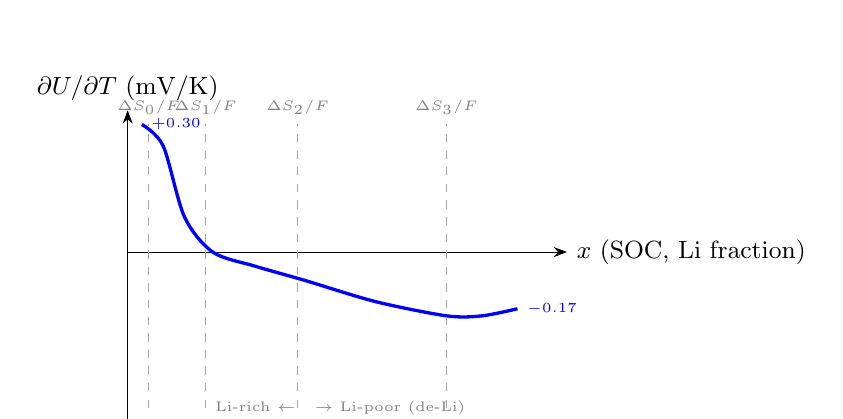
\begin{tikzpicture}[>=Stealth,font=\small,scale=0.9]
  \draw[->] (0,0) -- (6.2,0) node[right] {$x$ (SOC, Li fraction)};
  \draw[->] (0,-2.5) -- (0,2.0) node[above] {$\partial U/\partial T$ (mV/K)};
  % dS values for 4 transitions at approximate x positions
  % x ~ 0.08 (+29 mV/K equiv ~0.30), x~0.20 (0), x~0.40 (-0.052), x~0.70 (-0.166)
  % scale: 1 unit = ~0.13 mV/K  so 0.30 mV/K ~ 2.3u; just use scaled cartoon
  \draw[blue,very thick,smooth,tension=0.5]
    plot coordinates {(0.2,1.8)(0.5,1.5)(0.8,0.5)(1.2,0.0)(1.8,-0.2)
                      (2.5,-0.4)(3.5,-0.7)(4.5,-0.9)(5.0,-0.9)(5.5,-0.8)};
  % Mark transition centers
  \foreach \xc/\lb in {0.3/{$\Delta S_0/F$},1.1/{$\Delta S_1/F$},
                        2.4/{$\Delta S_2/F$},4.5/{$\Delta S_3/F$}}
    \draw[dashed,gray!70] (\xc,-2.2)--(\xc,1.8) node[above,gray,font=\tiny]{\lb};
  % Annotations
  \node[blue,right,font=\tiny] at (0.2,1.8) {$+0.30$};
  \node[blue,right,font=\tiny] at (5.5,-0.8) {$-0.17$};
  \node[font=\tiny,gray] at (3.0,-2.2) {Li-rich $\leftarrow$\quad$\rightarrow$ Li-poor (de-Li)};
\end{tikzpicture}
\caption{겹침 가중 모델의 $\partial U_\oc/\partial T(x)$ 개략 모양(흑연 4 전이, 단순식 기준).
  전이 경계에서 \emph{연속 블렌드} --- 계단 불연속 없음.
  Li-poor 쪽 양의 값($+0.30$ mV/K)이 stage 4$\to$3 의 큰 $\Delta S=+29$ J mol$^{-1}$K$^{-1}$ 를 반영.
  Li-rich 쪽 음의 값($-0.17$ mV/K)이 stage 2$\to$1 의 $\Delta S=-16$ J mol$^{-1}$K$^{-1}$ 에서 온다.}
\label{fig:dUdT_blend}
\end{figure}

\subsection{파생 B: 이중계산 금지}\label{sec:double_count}

식~\eqref{eq:weighted_dSdT} 에서 $\Delta S_{\rxn,j}$ 는 \emph{중심 표준값}이다
($\xi_j=1/2$, config$=0$).
봉우리 내부 $x$-의존은 logistic 폭 $w=RT/F$ 가 이미 제공한다 --- 이것이 배위 항
$R\ln[(1-\xi)/\xi]$ 이다.

\begin{warnbox}
\textbf{이중계산 B 금지}: 식~\eqref{eq:Stotal} 에서 $\Delta S^0_j$ 는 전이 중심에서
측정·피팅한 표준 반응 엔트로피(vib+electronic 기여 포함 중심값)이다. 여기에 config
항 $R\ln[(1-\xi)/\xi]$ 를 \emph{별도로 또 더하는 것}은 이중계산이다.
둘은 같은 식의 별개 항이며, config 는 분포($w$)가 자동으로 제공한다
(중심값에 config 를 수동으로 포함시키지 말 것).
\end{warnbox}

완전식에서의 완전한 표현은
\begin{equation}
  \frac{\partial U_\oc}{\partial T}(x)
  = \frac{\sum_j Q_j\,g_j\bigl(\Delta S_j/F + z_j R/F\bigr)}{\sum_j Q_j g_j}\,,
  \qquad z_j \equiv \frac{U_\oc(x)-U_j}{w_j}\,,
  \label{eq:full_dUdT}
\end{equation}
여기서 $z_j R/F$ 가 배위 항이다. $\xi_j=1/2$($U_\oc=U_j$)에서 $z_j=0$ → config=0 → 표준값 회수.

% ====================================================================
\section{상호작용과 유효 폭 $w_\eff(\Omega)$}\label{sec:weff}
% ====================================================================

\subsection{파생 C: 평균장 정규용액 기울기}

Bragg--Williams 식~\eqref{eq:BW} 에서 화학 퍼텐셜 편차
$\partial g/\partial\theta=RT\ln[\theta/(1-\theta)]+\Omega(1-2\theta)$ 를 $\theta$ 로
미분하면 등온선 기울기는
\begin{equation}
  \frac{\dd V_\eq}{\dd\xi} \;=\; \frac{RT}{F}\left[\frac{1}{\xi(1-\xi)}-\frac{2\Omega}{RT}\right]\,.
  \label{eq:iso_slope}
\end{equation}
$\xi=1/2$ (봉우리 중심)에서 $4[RT/(4F)-\Omega/(2F)]=(RT-\Omega/2)/F\cdot4 \to (4RT-2\Omega)/F$.
전이 봉우리 폭(반높이 반너비)은 $\xi=1/2$ 중심 기울기 역수에 비례하므로, 유효 폭은
\begin{equation}
  \boxed{\;w_\eff \;=\; \frac{w}{1-\Omega/(2RT)}\;,\quad w=\frac{RT}{F}\,.}
  \label{eq:weff}
\end{equation}
$\Omega>0$(척력): $w_\eff>w$ → 봉우리 넓어짐($\Delta S$ 봉우리 완만).
$\Omega<0$(인력): $w_\eff<w$ → 봉우리 좁아짐($\Delta S$ 봉우리 예리).
$\Omega\to2RT$: $w_\eff\to\infty$ → 봉우리 완전 평탄(상분리 임계, plateau).

온도 의존: $\Omega$ 자체가 약한 $T$ 의존($\partial\Omega/\partial T\ne0$)이면
$\partial w_\eff/\partial T$ 가 $\partial U/\partial T$ 에 2차 기여를 추가한다
(일반적으로 소수, 그러나 $\Omega$가 $T$ 에 민감한 계에서는 명시 필요).

\begin{figure}[h]
\centering
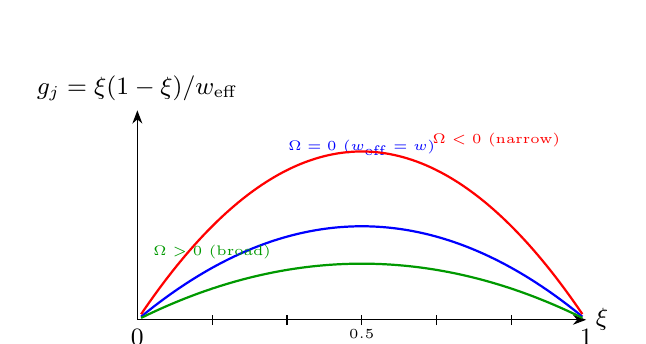
\begin{tikzpicture}[>=Stealth,font=\small,scale=0.95]
  \draw[->] (0,0) -- (6.0,0) node[right] {$\xi$};
  \draw[->] (0,0) -- (0,2.8) node[above] {$g_j=\xi(1-\xi)/w_\eff$};
  % Ideal Omega=0
  \draw[blue,thick,domain=0.05:5.95,samples=100]
    plot(\x, {5*(\x/6)*(1-\x/6)/0.9 * 0.9});
  \node[blue,font=\tiny] at (3,2.3) {$\Omega=0$ ($w_\eff=w$)};
  % Repulsive: broader
  \draw[green!60!black,thick,domain=0.05:5.95,samples=100]
    plot(\x, {5*(\x/6)*(1-\x/6)/1.5 * 0.9});
  \node[green!60!black,font=\tiny] at (1.0,0.9) {$\Omega>0$ (broad)};
  % Attractive: narrower
  \draw[red,thick,domain=0.05:5.95,samples=100]
    plot(\x, {5*(\x/6)*(1-\x/6)/0.5 * 0.9});
  \node[red,font=\tiny] at (4.8,2.4) {$\Omega<0$ (narrow)};
  \foreach \x in {1,2,3,4,5} \draw (\x,-0.07)--(\x,0.07);
  \node[below,font=\tiny] at (3,0) {$0.5$};
  \node[below] at (0,0) {$0$}; \node[below] at (6,0) {$1$};
\end{tikzpicture}
\caption{Bragg--Williams 상호작용이 dQ/dV 봉우리 형태 $g_j$ 에 미치는 영향.
  척력($\Omega>0$)은 봉우리를 넓히고, 인력($\Omega<0$)은 좁히며, $\Omega\to2RT$ 에서 평탄해진다.
  같은 $x$ 폭에서 좁은 봉우리는 더 가파른 $\partial U/\partial T$ 변동을 준다.}
\label{fig:weff}
\end{figure}

% ====================================================================
\section{히스테리시스 하 가역/비가역 분리}\label{sec:hys}
% ====================================================================

\subsection{파생 D: 분기별 엔트로피 계수}

흑연 OCV 는 충방전 이력의존(준안정 stacking, stage~II 무질서)이어서~\cite{hysteresis2018},
방전(dis, $d$)과 충전(ch, $c$) 분기의 전이 중심이
$U_j^{(d)}=U_j+\tfrac12\Delta U_j^\hys$ 와 $U_j^{(c)}=U_j-\tfrac12\Delta U_j^\hys$ 로
어긋난다. 각 분기에서 식~\eqref{eq:weighted_dSdT} 를 적용하면
\begin{equation}
  \frac{\partial U_\oc^{(d)}}{\partial T} =
  \frac{1}{F}\frac{\sum_j Q_j g_j^{(d)}\,\Delta S_{\rxn,j}}{\sum_j Q_j g_j^{(d)}}\,,
  \quad
  \frac{\partial U_\oc^{(c)}}{\partial T} =
  \frac{1}{F}\frac{\sum_j Q_j g_j^{(c)}\,\Delta S_{\rxn,j}}{\sum_j Q_j g_j^{(c)}}\,,
  \label{eq:hys_branches}
\end{equation}
여기서 $g_j^{(d/c)}=\xi_j^{(d/c)}(1-\xi_j^{(d/c)})/w_j$ 는 분기 봉우리 모양이다.

\subsection{가역 발열(평균)과 비가역 손실(hiys gap) 분리}

열역학적 \textbf{가역 엔트로피 계수}는 두 분기의 평균으로 정의한다:
\begin{equation}
  \frac{\partial U^\rev}{\partial T} \;=\;
  \frac12\left(\frac{\partial U^{(d)}}{\partial T}+\frac{\partial U^{(c)}}{\partial T}\right)\,.
  \label{eq:Urev}
\end{equation}
이로부터 \emph{가역 발열}은 식~\eqref{eq:qrev} 에 $\partial U^\rev/\partial T$ 를 대입한 값이다.

히스테리시스 gap $\Delta U_j^\hys$ 자체는 준안정 상전이에 동반한 \emph{비가역 엔트로피 생성}이며,
전류 방향마다 $I\,\Delta U^\hys$ 에 비례하는 비가역열로 분리된다. 이 두 성분을 혼동하면
가역 발열을 과대/과소 추정한다.

\begin{warnbox}
히스 분기 평균(식~\eqref{eq:Urev})이 \emph{가역} 기준인 것은, 두 준안정 상태
사이의 중간이 진정한 평형에 가장 가깝기 때문이다. 그러나 이 근사는 히스 gap 이
열역학 기여를 완전히 수렴시켰을 때만 정확하며, 나머지 경로의존 불확실도는
\S\ref{sec:limit} 에서 다룬다.
\end{warnbox}

% ====================================================================
\section{극한 검산과 근사 타당성 판정}\label{sec:limits}
% ====================================================================

\subsection{파생 I: 여섯 극한}

\begin{table}[h]
\centering\small
\renewcommand{\arraystretch}{1.25}
\caption{$\partial U/\partial T$ 극한 및 코너 검산.}
\label{tab:limits}
\begin{tabular}{l l l}
\toprule
극한 & $\partial U/\partial T$ 거동 & 물리 해석 \\
\midrule
$\xi\to0$ (만충) & config $\to-\infty$ & 정렬 강요 → 큰 음의 부분몰 ΔS \\
$\xi\to1$ (희박) & config $\to+\infty$ & Li 희박 혼합 이득 → 큰 양의 ΔS \\
$\xi=1/2$ (중심) & $=\Delta S_{\rxn,j}/F$ & config$=0$, 표준값 그대로 회수 \\
$\Omega\to2RT^-$ & $w_\eff\to\infty$, plateau & 상분리 임계; ∂U/∂T 평탄·불연속 \\
단일 봉우리 & $=\Delta S_{\rxn,j}/F$ + config & 겹침 없음 → 단일 전이로 환원 \\
고온 & $\Delta S_\elec\propto T$ 우세화 & Sommerfeld FD 분포; LCO MIT 게이트 \\
\bottomrule
\end{tabular}
\end{table}

\subsection{"$\Delta S_{\rxn,j}$ 전이당 상수" 근사의 타당성}

식~\eqref{eq:weighted_dSdT} 는 $\Delta S_{\rxn,j}$ 를 전이별 \emph{상수}로 둔다.
이 근사가 타당한 조건:
\begin{enumerate}[leftmargin=1.6em,itemsep=2pt]
\item vib 및 electronic 기여가 전이 폭 내에서 천천히 변할 때 (전이 폭 $\sim w$ 스케일에서 완만).
\item 측정 $\partial U/\partial T(x)$ 비선형은 (i)~겹침 가중과 (ii)~봉우리-내부 config 두 출처로
  \emph{자동 생성}되며, $\Delta S_{\rxn,j}$ 를 $x$-함수로 굳이 만들 필요가 없다.
\item 예외: MIT 게이트가 단일 전이 폭 안에서 $g(E_F)$ 를 급변시키는 LCO T1 전이 등.
  이 경우 $\Delta S_\elec(x)$ 를 명시 $x$-함수로 두어야 한다(Ch1 v9 확장의 의미).
\end{enumerate}

수치검증~\cite{verif42}: 모델 내 비선형 $\partial U/\partial T(x)$ 가 상수 $\Delta S_{\rxn,j}$
만으로 부동소수점 수준에서 완벽 재현됨 → 근사 타당성 확인.

% ====================================================================
\section{흑연 staging 엔트로피 프로파일 — 문헌값과 Chapter 1 정합}\label{sec:profile}
% ====================================================================

$\Delta S_{\rxn,j}$ 가 가역 발열을 결정하므로, 흑연의 측정 엔트로피 프로파일이 검증 기준이다.

\begin{itemize}[leftmargin=1.4em,itemsep=2pt]
\item 저 Li 분율($x<0.2$)에서 $\Delta S>0$(configurational 기여), 고 분율에서 $\Delta S<0$
  (vibrational 기여) — Reynier, Yazami, Fultz~\cite{reynier2003}; Allart 등~\cite{allart2018}.
\item 정량 전극 분리: $\Delta S\approx+29$ J\,mol$^{-1}$K$^{-1}$ @$x=0.08$,
  $-5\sim-16$ J\,mol$^{-1}$K$^{-1}$ @$x>0.5$~\cite{allart2018}.
\item MCMB 흑연 $\partial U/\partial T\approx+3\sim4$ mV/K @저-$x$,
  $\sim0.2$ SOC 부근 부호 반전~\cite{msmr_partII}.
\item stage\,2$\to$1 ($x\approx0.5$) 에서 엔트로피 급재증가(이상 거동)~\cite{reynier2003,allart2018}.
\end{itemize}

\begin{srcbox}
\textbf{Chapter~1 정합(정량).} Ch1 \texttt{GRAPHITE\_STAGING\_LIT} 의 전이별
$\Delta S_{\rxn,j}=+29\to0\to-5\to-16$ J\,mol$^{-1}$K$^{-1}$ 은 Allart 등~\cite{allart2018}
과 \emph{부호·규모 정량 일치}한다($+29$ @저-$x$, $-16$ @$x>0.5$ 정확 대응).
Ch1 의 엔트로피 값은 문헌 근거에 닿아 있으며, 가역 발열 사슬의 입력이 임의값이 아님을
뒷받침한다. 표~\ref{tab:ds} 참조.
\end{srcbox}

\begin{table}[h]
\centering\small
\renewcommand{\arraystretch}{1.2}
\caption{Chapter~1 전이별 $\Delta S_{\rxn,j}$ ↔ 문헌 흑연 $\Delta S(x)$ (Allart 등~\cite{allart2018}, 전극 분리).}
\label{tab:ds}
\begin{tabular}{l c c c}
\toprule
전이 & $x$ 범위 & Ch1 $\Delta S_{\rxn,j}$ [J\,mol$^{-1}$K$^{-1}$] & 문헌 $\Delta S(x)$ \\
\midrule
$4\!\to\!3$ & 0.08--0.16 & $+29.0$ & $+29$ @\,$x=0.08$ (정확) \\
$3\!\to\!2\mathrm{L}$ & 0.16--0.25 & $0.0$ & 중간 하강 구간 $0\!\to\!-16$ (범위) \\
$2\mathrm{L}\!\to\!2$ & 0.25--0.50 & $-5.0$ & 중간 하강 구간 (범위) \\
$2\!\to\!1$ & 0.50--1.00 & $-16.0$ & $-16$ @\,$x>0.5$ (정확) \\
\bottomrule
\end{tabular}
\smallskip

{\footnotesize $x$-경계는 $1{:}1$ 대응이 아니다: 양 끝($+29$ @저-$x$, $-16$ @$x>0.5$)은
정확 대응하고, 중간 두 전이는 $\Delta S$ 하강 구간 안에 놓인다(해상도 차이, 부호·추세 일관).}
\end{table}

% ====================================================================
\section{반응 엔트로피 vs 활성화 엔트로피 — 혼동 금지}\label{sec:caveat}
% ====================================================================

가역 발열의 핵심 함정은 두 엔트로피의 혼동이다. \textbf{반응 엔트로피}
$\Delta S_{\rxn,j}=F\,\partial U_j/\partial T$ 는 \emph{평형} 상태함수로,
가역열 식~\eqref{eq:qrev} 에 들어간다. \textbf{활성화 엔트로피} $\Delta S_{a,j}$ 는
Chapter~1 의 동역학 꼬리(Eyring 속도상수 prefactor 의 온도의존)로,
비가역열을 지배한다. 차원은 같으나 물리가 다르다~\cite{msmr_partI}.

% ====================================================================
\section{가역 발열 합산 — 분포 재배열 열}\label{sec:qrev_synthesis}
% ====================================================================

\subsection{가역 발열 = 분포 재배열 열}

식~\eqref{eq:weighted_dSdT} 와 \eqref{eq:qrev} 를 결합하면
\begin{equation}
  \boxed{\;
  \dot Q_\rev = -\frac{IT}{F}\,
  \frac{\sum_j Q_j g_j(x)\,\Delta S_{\rxn,j}}{\sum_j Q_j g_j(x)}\,.
  \;}
  \label{eq:qrev_final}
\end{equation}
이것이 식~\eqref{eq:qrev} 의 닫힌 형태다. $\dot Q_\rev$ 의 물리적 의미:
충/방전 시 Li(+전자) 집단이 SOC $(x)$ 에서 $x+\dd x$ 로 이동할 때,
분포 $\{\xi_j\}$ 가 재배열되면서 방출(또는 흡수)하는 열이다.

\subsection{SOC별 흡발열 교대}

식~\eqref{eq:qrev_final} 에서 $\overline{\Delta S}(x)>0$ 이면(저-$x$, 저율 방전)
$\dot Q_\rev>0$ (발열). $\overline{\Delta S}(x)<0$ 이면(고-$x$, 고충전) $\dot Q_\rev<0$ (흡열).
흑연 음극의 흡발열 교대:

\begin{itemize}[leftmargin=1.4em,itemsep=2pt]
\item 방전 초기($x<0.2$, Li-poor, stage 4$\to$3): 양의 $\Delta S$ → 방전 시 발열 기여.
\item 방전 중반($x\approx0.5$, stage 2$\to$1): 가장 큰 음의 $\Delta S=-16$ J mol$^{-1}$K$^{-1}$
  → 방전 시 강한 흡열(calorimetry 직접 관측~\cite{standardised2024} 과 정합).
\end{itemize}

\subsection{다온도 $dQ/dV$ 피팅과의 연결}

사슬: 여러 $T_k$ 에서 $dQ/dV$ → Ch1 모델 동시 피팅 → $U_j(T_k)$ 기울기 →
$\Delta S_{\rxn,j}$ → 식~\eqref{eq:qrev_final} → $\dot Q_\rev(x,T)$.

MSMR~\cite{msmr_partI,msmr_partII} 은 흑연 OCV 를 반응별 항 합으로 보고,
각 반응 $U_j^0(T)$ 를 저차 다항으로 두어 $\partial U_j^0/\partial T$ 를 추정한다.
이는 Ch1 의 전이별 logistic 구조와 직접 대응한다.

\textbf{피팅 함정.} 저율 준평형 데이터(고율은 동역학 오염), 평활 폭 최소화(과평활
→ 폭 양의 편향), 분극·히스 분리 후 $\partial U/\partial T$ 추정~\cite{msmr_partI,msmr_partII}.

% ====================================================================
\section{한계와 공백 (정직)}\label{sec:limit}
% ====================================================================

\begin{enumerate}[leftmargin=1.6em,itemsep=3pt]
\item \textbf{$dQ/dV(T)$ 직접 추정 정확도}: 실데이터 round-trip 으로만 확정(후속).
\item \textbf{히스 하 경로의존 $\partial U/\partial T$ 불확실도}: 정량 미확보.
  $\Delta U^\hys$ 의 $T$ 의존이 식~\eqref{eq:hys_branches} 에 2차 기여를 줄 수 있다.
\item \textbf{Bragg--Williams 평균장 한계}: 실제 흑연은 비균일 격자·층간 상관이 있어
  $\Omega$ 의 공간 분포를 단일 수로 대표하는 것이 근사임.
\item \textbf{electronic 엔트로피 흑연 음극}: $\Delta S_\elec\approx0$ 가정은
  흑연 금속성이 충분히 강할 때. 저-$x$ 희석 한계($x<0.05$)에서 부분 절연체 거동
  가능 --- 미정량.
\item \textbf{Electrochimica Acta 2019~\cite{occupation2019} prototype}: 원문 식 미확보(유료).
  방법 수준만 인용.
\end{enumerate}

% ====================================================================
\section*{맺음 — 분포 전개의 사슬}
\addcontentsline{toc}{section}{맺음}
% ====================================================================

이 장은 격자기체 grand-canonical 분배함수에서 출발하여 다음 사슬을 닫았다:
\[
  Z_1 \;\to\; \langle n\rangle=\xi_{\eq,j}
  \;\to\; S_\config=-R\sum p\ln p
  \;\to\; \frac{\partial U}{\partial T}(x)
  \;\to\; \dot Q_\rev=-IT\,\frac{\partial U}{\partial T}\,.
\]
핵심 결과:
\begin{itemize}[leftmargin=1.4em,itemsep=2pt]
\item Ch1 의 logistic 함수는 격자기체 점유 분포이고, 그 폭 $w=RT/F$ 는 배위 엔트로피를 담는다.
\item 관측 $\partial U_\oc/\partial T(x)$ 는 세 분포(격자기체 config, 포논 BE, 전자 FD)의 합이다.
\item 겹침 가중식(파생 A)은 연속 블렌드를 준다(계단 불연속 없음 --- 수치검증~\cite{verif42} PASS).
\item 이중계산 B: $\Delta S^0_j$ = 중심 표준값, 배위 항은 분포가 자동 제공 --- 별도 가산 금지.
\item $w_\eff(\Omega)=w/(1-\Omega/2RT)$ 는 상호작용이 봉우리 폭·$\partial U/\partial T$ 형태를 변조하는 방식을 요약한다.
\item 가역 발열은 분포의 SOC 재배열이 유발하는 열이며, 흡발열 교대는 $\overline{\Delta S}(x)$
  의 부호 변화에서 직접 나온다.
\end{itemize}

\textbf{다음}: (i) 실데이터 다온도 $dQ/dV$ round-trip 으로 $\Delta S_{\rxn,j}$ 정량 실증,
(ii) $w_\eff(\Omega)$ 의 온도 의존 정량(동적 Bragg--Williams),
(iii) Ch1 v9 통합(가역/비가역 발열 한 인과 사슬로).

% ====================================================================
\begin{thebibliography}{99}

\bibitem{bernardi1985}
D. Bernardi, E. Pawlikowski, J. Newman,
``A General Energy Balance for Battery Systems,''
\emph{J. Electrochem. Soc.} \textbf{132}(1), 5--12 (1985).
DOI: 10.1149/1.2113792.

\bibitem{newman2004}
J. Newman, K. E. Thomas-Alyea,
\emph{Electrochemical Systems}, 3rd ed., Wiley (2004).

\bibitem{reynolds_huggins}
C. M. Huggins,
\emph{Advanced Batteries: Materials Science Aspects},
Springer (2009). [Lattice-gas grand-canonical OCV derivation.]

\bibitem{bazant_lattice}
M. Z. Bazant,
``Theory of chemical kinetics and charge transfer based on nonequilibrium thermodynamics,''
\emph{Acc. Chem. Res.} \textbf{46}(5), 1144--1160 (2013).
DOI: 10.1021/ar300145c.

\bibitem{reynier2003}
Y. Reynier, R. Yazami, B. Fultz,
``The entropy and enthalpy of lithium intercalation into graphite,''
\emph{J. Power Sources} \textbf{119--121}, 850--855 (2003).
DOI: 10.1016/S0378-7753(03)00285-4.

\bibitem{allart2018}
D. Allart \emph{et al.},
``Model of Lithium Intercalation into Graphite by Potentiometric Analysis with
Equilibrium and Entropy Change Curves of the Graphite Electrode,''
\emph{J. Electrochem. Soc.} \textbf{165}(2), A380 (2018).
DOI: 10.1149/2.1251802jes.

\bibitem{occupation2019}
``Transitions of lithium occupation in graphite: A physically informed model in the
dilute lithium occupation limit supported by electrochemical and thermodynamic measurements,''
\emph{Electrochimica Acta} (2019).
DOI: 10.1016/j.electacta.2019.135634.
[방법 수준 인용 — 원문 식 미확보.]

\bibitem{chemmater2015}
``Intercalation Compounds from LiH and Graphite: Relative Stability of Metastable Stages\ldots,''
\emph{Chem. Mater.} \textbf{27} (2015).
DOI: 10.1021/acs.chemmater.5b00235.
[형성 $\Delta H$ calorimetry — abstract tier.]

\bibitem{jpcc2021}
``Thermodynamic Analysis of Li-Intercalated Graphite by First-Principles with
Vibrational and Configurational Contributions,''
\emph{J. Phys. Chem. C} \textbf{125} (2021).
DOI: 10.1021/acs.jpcc.1c08992.
[abstract tier.]

\bibitem{msmr_partI}
``Quantifying the Entropy and Enthalpy of Insertion Materials for Battery Applications
Via the Multi-Species, Multi-Reaction Model,''
\emph{J. Electrochem. Soc.} (2024).
DOI: 10.1149/1945-7111/ad1d27.

\bibitem{msmr_partII}
``Quantifying the Temperature Dependence of the MSMR Model Part II:
Estimation of Entropy Coefficient for Meso-Carbon Micro-Bead Graphite,''
\emph{J. Electrochem. Soc.} (2024).
DOI: 10.1149/1945-7111/ad70d9.

\bibitem{standardised2024}
``A Standardised Potentiometric Method for the Effective Parameterisation of
Reversible Heating in a Lithium-Ion Cell,''
\emph{J. Electrochem. Soc.} (2024).
DOI: 10.1149/1945-7111/ad4918.

\bibitem{hysteresis2018}
``Uncertainties in entropy due to temperature path dependent voltage hysteresis
in Li-ion cells,''
\emph{J. Power Sources} (2018).
DOI: 10.1016/j.jpowsour.2018.05.060.

\bibitem{verif42}
수치검증 스크립트 \texttt{verify\_v6\_clean.py}, Ch2 v4 파생 A 검증,
\texttt{42\_numerical\_verification.md} (2026-06-30).
[내부 문서 — 외부 미공개.]

\end{thebibliography}

\end{document}
